% !TeX root = ../main.tex

\section{Background}
\label{sec:bg}


\subsection{Efficiency in LLM-Based Code Processing}
\label{subsec:token_electricity}

% TODO： 这个部分讲：
% 1. 模型用于Code Processing：generation， etc
% 2. 模型产生的code，有很多token，具体，一个issue问题解决，可能需要XXX token
% 3. token有很多冗余的
% 4. 冗余token 的问题解决，可以提升推理速度，同时帮助节省多少多少token成本。

Large language models (LLMs) are now used for a wide range of code-processing tasks. At the function level, HumanEval asks a model to generate function implementations from signatures and docstrings~\cite{chen2021codex}, while CodaMosa uses language models to support test generation~\cite{lemieux2023codamosa}. At the repository level, RepoBench evaluates code completion that depends on information from other files~\cite{liu2023repobench}, and SWE-bench asks systems to resolve real GitHub issues by producing patches for existing repositories~\cite{jimenez2024swebench}. These tasks may require the model to process functions, interfaces, usage examples, tests, and dependencies distributed across multiple files.

The resulting token cost can be substantial. SWE-Effi evaluated software-engineering agents on 50 stratified SWE-bench Verified issues and reported that AutoCodeRover with Qwen3-32B processed an average of 55.5K input tokens and 20.4K output tokens per issue attempt. Under the same model, SWE-Agent processed 440.2K input tokens and 41.0K output tokens~\cite{fan2025sweeffi}. Thus, a single real-world issue attempt can involve tens or even hundreds of thousands of tokens, depending on the workflow. More tokens increase computation, memory use, latency, and serving cost, while also consuming space that could hold other useful repository context.

Source code is designed primarily for people to write, read, and maintain. It therefore contains indentation, line organization, delimiters, fixed syntactic forms, and recurring code idioms that improve human readability but can expand into multiple model tokens. Some of this information is predictable from the programming language grammar or repeats across programs, while identifiers, literals, and program-specific expressions carry less replaceable information. Treating all of these elements identically leaves recoverable redundancy in the model input.

A denser code representation can reduce this redundancy after the relevant context has been selected. Shorter representations lower the number of tokens processed during training and inference, reduce latency and computational cost, and leave more of the context window available for useful program information. These benefits, however, require the representation to preserve the structure and content needed to recover executable code and to remain learnable by the model. This motivates reversible token reduction designed specifically for generative code processing.

\subsection{Motivating Example}


% 第一段，讲核心相关工作simpy token sugar原理
% 第二段，引入normalized例子，告诉别人还有reduction空间
% 第三段，引入conditional例子，告诉别人如果不做conditional，效果会适得其反，影响LLM推理准确率

SimPy~\cite{simpy2024} and TokenSugar~\cite{tokensugar2024} demonstrate two complementary ways to shorten source code. SimPy redesigns the Python surface grammar to reduce layout, delimiters, and other fixed syntactic forms~\cite{simpy2024}, whereas TokenSugar replaces recurring multi-token code patterns with compact shorthand tokens~\cite{tokensugar2024}. Consider the following Python function:

\begin{center}
\setlength{\fboxsep}{6pt}
\fbox{%
  \begin{minipage}{0.88\columnwidth}
\ttfamily\small
def collect(items, errors):\\
\hspace*{1em}result = []\\
\hspace*{1em}for item in items:\\
\hspace*{2em}if item is None:\\
\hspace*{3em}errors.append(item)\\
\hspace*{3em}continue\\
\hspace*{2em}result.append(item)\\
\hspace*{1em}return result
  \end{minipage}%
}
\end{center}

Its indentation and block organization support human readability, while \texttt{errors.append(item)} and \texttt{result.append(item)} instantiate the same recurring call structure. The example therefore contains both grammar-level redundancy and repeated idiomatic structure.

\tool handles these two forms within a unified representation. Normalization converts indentation, line organization, block boundaries, and selected fixed syntax into a compact surface that can be reconstructed from Python grammar and decoder state. Program-specific content, including \texttt{items}, \texttt{errors}, \texttt{result}, and \texttt{item}, remains explicit. Hybrid Idioms Shorthanding then operates on this normalized surface. For example, the two calls can share one shorthand schema, written schematically as \texttt{<append>(receiver, argument)}, with their different receivers and arguments retained as captures. Normalization therefore not only reduces structural tokens directly, but also provides a stable surface on which recurring idioms can be collected and represented consistently.

A reversible codec could replace both eligible calls because either shorthand can be decoded correctly. However, this uniform policy assumes that the two occurrences are equally suitable for the target model. Their surrounding control flow and prediction contexts differ, so replacing them may impose different adaptation costs even though they use the same shorthand schema. Conditional Attention evaluates the occurrences separately. It may retain \texttt{errors.append(item)} in expanded form while encoding \texttt{result.append(item)} with the shorthand, or make the opposite decision, according to the model-derived signal. This example motivates occurrence-level selection: the codec determines which transformations are valid, while the model signal determines where an eligible transformation is applied.


\subsection{Compression Opportunities in Source Code}
\label{subsec:rationale}

To characterize the theoretical and practical boundaries of code compression, we analyze token composition across three diverse Python corpora: CodeSearchNet, our GitHub-Code-Clean corpus, and our curated high-quality repository corpus. We classify tokens into seven functional classes according to their roles in source text and the abstract syntax tree (AST), and organize them into three tiers with different compression opportunities and risks. Figure~\ref{fig:taxonomy} shows the aggregate distribution, and Table~\ref{tab:taxonomy} summarizes the role of each class.

\begin{figure}[!t]
  \centering
  \definecolor{taxblue}{HTML}{4E79A7}
  \definecolor{taxorange}{HTML}{F28E2B}
  \definecolor{taxgreen}{HTML}{59A14F}
  \definecolor{taxred}{HTML}{E15759}
  \definecolor{taxpurple}{HTML}{B07AA1}
  \definecolor{taxteal}{HTML}{76B7B2}
  \definecolor{taxyellow}{HTML}{EDC948}
  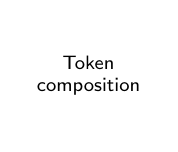
\begin{tikzpicture}[
    scale=0.78,
    every node/.style={font=\scriptsize},
    taxslice/.style={draw=white, line width=0.8pt}
  ]
    \pie[
      text=legend,
      hide number,
      sum=99.9,
      radius=1.65,
      rotate=90,
      style={taxslice},
      color={taxblue, taxorange, taxgreen, taxred, taxpurple, taxteal, taxyellow}
    ]{
      10.5/Layout (10.5\%),
      21.9/Punctuation (21.9\%),
      5.3/Comments (5.3\%),
      4.1/Keywords (4.1\%),
      4.4/Operators (4.4\%),
      29.5/Identifiers (29.5\%),
      24.2/Literals (24.2\%)
    }
    \fill[white] (0,0) circle (0.78);
    \node[align=center, font=\sffamily\scriptsize] at (0,0) {Token\\composition};
  \end{tikzpicture}
  \vspace{-5pt}
  \caption{Token taxonomy across the analyzed Python corpora. Tiers 1 and 2 are the primary compression targets, while Tier 3 carries program-specific content.}
  \Description{Pie chart showing layout 10.5 percent, punctuation 21.9 percent, comments 5.3 percent, keywords 4.1 percent, operators 4.4 percent, identifiers 29.5 percent, and literals 24.2 percent.}
  \label{fig:taxonomy}
\end{figure}

\begin{table}[!t]
    \centering
    \footnotesize
    \setlength{\tabcolsep}{3pt}
    \renewcommand{\arraystretch}{1.05}
    \caption{Token taxonomy and aggregate distribution in the analyzed Python corpora.}
    \vspace{-5pt}
    \label{tab:taxonomy}
    % \begin{tabularx}{\columnwidth}{@{}llr>{\raggedright\arraybackslash}X@{}}

       \begin{tabular}{>{\raggedright\arraybackslash}p{1cm}
                >{\centering\arraybackslash}p{3cm}
                >{\raggedright\arraybackslash}p{1cm}
                >{\centering\arraybackslash}p{5cm}
                }
    \toprule
    \textbf{Tier} & \textbf{Functional class} & \textbf{Ratio} & \textbf{Compression property} \\
    \midrule
    1 & Formatting and layout & 10.5\% & Reconstructable layout markers \\
      & Syntax punctuation & 21.9\% & Repeated syntactic delimiters \\
      & Comments & 5.3\% & Non-executable documentation \\
    \midrule
    2 & Keywords & 4.1\% & Predictable structural operations \\
      & Operators & 4.4\% & Recurring symbolic operations \\
    \midrule
    3 & Identifiers & 29.5\% & Program-specific names \\
      & Literals & 24.2\% & Program-specific values \\
    \bottomrule
    \end{tabular}
\end{table}

This distribution reveals a hierarchy of compressibility and associated risks:

\begin{enumerate}[leftmargin=*]
    \item \textbf{High-yield redundancy (Tier 1).} Layout, punctuation, and comments account for 37.7\% of the observed tokens. Much of this material supports human-readable presentation or repeats structural information that a deterministic decoder can reconstruct. It therefore offers the largest immediate opportunity, although not every token in the tier can be removed under a reversible contract.
    \item \textbf{Predictable semantic space (Tier 2).} Keywords and operators account for another 8.5\%. They frequently occur in rigid syntax and recurring idioms, such as \texttt{for \_ in range} and \texttt{if \_\_name\_\_ == "\_\_main\_\_"}, making complete multi-token structures suitable for fixed-vocabulary shorthands.
    \item \textbf{Sensitive logical payload (Tier 3).} Identifiers and literals account for 53.7\%. They carry program-specific names, values, and data-flow relationships. \tool therefore keeps them explicit unless a reversible pattern schema transports them as captures.
\end{enumerate}

\textbf{Compression opportunity bound.} Tiers 1 and 2 together occupy approximately 46.2\% of the analyzed token stream, giving a first-order upper bound near 46\% when identifiers and literals are left unchanged. This is an opportunity bound derived from token composition, not a claim that every tokenizer can realize a 46\% reduction. Some syntax must remain explicit or be re-encoded, comments may be preserved, and shorthand symbols, captures, and boundaries all consume tokens. The realized gain therefore depends on the tokenizer, corpus, registry size, and reversible representation cost.

We test this estimate in RQ1 by encoding real programs and counting them with the same tokenizer before and after encoding. Normalization shortens recoverable structure, while Hybrid Idioms Shorthanding replaces repeated patterns that remain on the normalized surface. The measurements therefore show how these two forms of reduction complement each other and how much compression they achieve in practice.
